% !TEX root = DesignDoc.tex

\chapter{ROS Architecture}
\label{chap:rosarch}

In this chapter, list the nodes running and show an rqtplot or similar visualization. Provide reasons behind the choices made for the design, if algorithms were a strong point of the design.

\section{Nodes}

\begin{itemize}
\item{Node 1}
\item{Node 2}
\item{...}
\end{itemize}


Describe the node functions here in as many subsections as you have nodes.

\section{rqtplot}

%\begin{figure}[h]
%\centering
%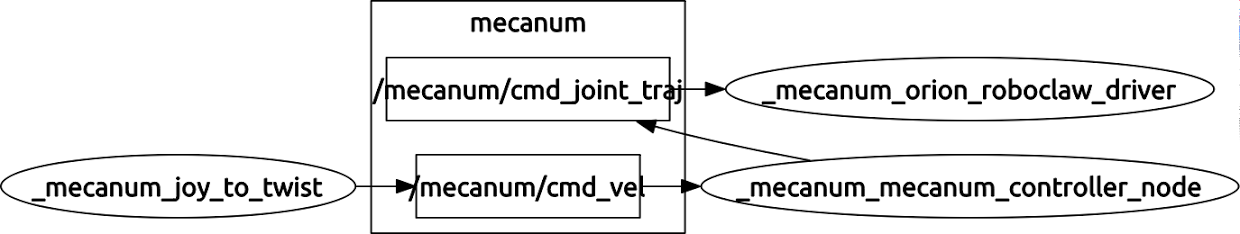
\includegraphics[width=\textwidth]{rqtplotmecanum.png}
%\label{fig:rqtplotmecanum}
%\caption{Mecanum rqtplot}
%\end{figure}

\section{Other Packages}

If you have any other important packages to note - simulators for instance - note them here.

\section{Other Files}

Supporting files, such as udev rules, service files, and the like, should be mentioned here.
